% !Mode:: "TeX:UTF-8"

\chapter[绪论]{绪论}[]
%7-8页
\section{课题研究背景及意义} 
近年来,许多国家致力于大力发展智能交通系统(ITS)[],以帮助实现高效的交通管理。智能交通系统是指将先进的传感器技术、实时信息技术、有线网络技术、无线网络通信技术、自动控制技术、RFID射频识别技术和计算机技术应用于整个交通运输管理体系,所建立的一种实时监控、控制和信息化管理系统。随着物联网技术的发展,智能交通在我国交通领域也有了较大的进展,诸如交通流量预测[]、旅行需求预测[]、交通拥堵检测[]等智能交通应用也得到了人们的重视,而这些智能交通应用可以有效地提高交通运输效率,缓解交通拥堵情况甚至避免极端事件的发生。例如,发生于2014年跨年夜上海外滩灯光秀活动的大型人员踩踏事故,据悉事故发生前当地的人流量超过100万人,这已远远超出了该地区人流量的正常水平,若有相关应用能及时地对当地人流量进行预测,那么就能提前进行人员疏散工作,避免悲剧的发生。但是,这些交通应用的正常运行往往依赖于大批量的正常数据,但是在实际的应用场景中,由于测量误差,检测技术的不成熟,数据损坏和设备故障等问题,都会造成收集到的数据不完整,这在一定程度上限制了智能交通的使用性能。因此,正确地处理不完整的数据,提升智能交通应用的预测能力,已经成为了智能交通领域的一个十分重要的研究方向。

根据数据中缺失点的分布以及缺失点之间的关系,一般将缺失情况分为三种模式\cite{little2019statistical},即随机缺失、完全随机缺失、非随机缺失。其中随机缺失是指缺失点的产生依赖于周围的值;完全随机缺失是随机缺失的特殊情况,指每个缺失点都完全独立于其他缺失值和观测值; 非随机缺失是指缺失值的产生依赖于其自身,通常由采集器长时间的设备故障造成。

大多数研究人员在使用含有缺失值的数据前,只是简单地将含缺失值的数据进行简单删除。但是这种做法会导致可用数据减少。交通数据是一种复杂的时空数据,具有复杂的时空特征,因而需要大批量的数据进行训练。这种简单删除的做法并不适用于交通数据的处理。Acuna[]等人也指出,若缺失值占比低于15%,可以通过删除法来解决,但是若缺失率超过15%,则需要仔细设计补全缺失值的方法以免对后期模型的训练结果产生过大影响。

目前,研究人员提出了很多针对于交通数据的缺失值填充算法,虽然也取得了一定的填充效果,但是,它们也存在明显的缺陷。
第一,大多数模型只是简单地关注于交通数据的空间特征,或者时间特征。但是交通数据作为一种复杂的时空数据,具有较强的时间依赖性和空间依赖性。
第二,目前的缺失值填充算法并没有对缺失值和存在值进行详细的区分,而是简单地将它们一并处理。这样的处理方案使得模型没有充分学习存在值的特征,容易造成模型的生成效果不佳。
第三,缺失值的存在会导致交通数据的时间分布特性发生变化,同时,对交通数据的空间分布特性也会产生影响。因此,使用普通的时间特征和空间特征提取方法去处理带有缺失值的交通数据很难得到理想的效果。
第四,以往的填充算法往往只适用于低缺失率的场景,在高缺失率的场景中,模型的填充能力往往很不如人意。

根据现有的研究资料可知,变分自编码器作为一种新型的深度生成神经网络,可以应用到交通数据的缺失值填充问题中。而且,变分自编码器具有很强的抗干扰能力,可以有效地提高模型的生成能力,因而,针对于带有缺失值的交通数据的时间特性和空间特性,在变分自编码器的基础上进行填充算法设计以实现时空特征推理的正确性,并能在高缺失率的情况下达到较低的填充误差,具有重要的实际价值和现实研究意义。

\section{国内外研究现状}
本小节将会阐述近年来交通领域关于缺失值填充算法的研究现状。根据本文研究内容,大致可以将其分为三类,分别是基于统计机器学习的填充算法、基于生成模型的填充算法和基于变分自编码器的缺失值处理方法。

\subsection{基于统计机器学习的缺失值填充算法研究现状}
基于统计学习的方法主要包括平均值、中值、线性回归(Linear regression, LR)和时间序列等。平均值和中值是最简单的基于统计学习的方法,但它们通常忽略交通状况的变化并降低插补性能,因此它们更适合交通数据平稳波动的情况。线性回归很容易应用,但它没有考虑交通数据的空间和时间特征,导致随着数据丢失率的增加和道路条件的复杂性而缺乏稳定性[]。线性回归仅确定历史观测值与未来流量之间的定量关系。交通数据具有动态的时间依赖性,不同区域的流量会相互影响,因此线性回归很难建模。时间序列插补[]可以充分利用历史数据来获得数据的时间分布特征,而当数据连续缺失时,它无法捕获时间相关性。
为了减少上述插补问题并提高实验精度,提出了各种基于机器学习的方法来填充缺失的交通数据,这些数据大致可分为两类:一类是使用AdaBoost回归和Ridge回归以及整合移动平均自回归模型(Autoregressive integrated moving average, ARIMA)以及其变体SARIMA等回归模型的预测方法。这些基于预测的方法往往只考虑了交通数据的时间相关性,却忽略了交通数据的空间相关性。第二种是插值方法,如k近邻方法(K-Nearest Neighbor, KNN)[12,13]、(Support Vector Regression, SVR)[14]、贝叶斯主成分分析(Bayesian Principal Component Analysis, BPCA)[15]和基于张量的插补方法(High Accuracy Low-rank Tensor Completion,HaLRTC)[16]。Li等人[12,13]使用KNN填充缺失的交通数据。首先,通过距离计算公式获得现有数据与缺失数据之间的距离,然后将k个最接近的数据平均为插补值。Tan等人[16]提出了一种基于张量的插补方法,该方法首先引入张量的概念来插补不完整的交通数据,并充分利用了时空信息。Cheng等人[17]利用了一种两步方法来重建时空缺失数据。Duan等人[18]提出了一种用于交通数据插补的去噪叠加自动编码器,同时考虑了时间和空间因素。为了提高估计值的准确性,Huang等人[19]提出了一种基于模糊C均值(FCM)和遗传算法(GA)的集成插补算法。首先获取缺失交通数据的粗粒度估计值,然后使用动态滑动窗口选择算法确定最相关的样本数据作为细粒度插补值。由于同时考虑了交通数据的时空相关性,该方法减少了数据连续缺失时的影响,提高了插补精度。大多数基于机器学习的方法考虑了交通数据的时空相关性,优于基于统计学习的方法,但它们依赖于相邻数据,通常假设缺失数据的位置是固定的,而实际缺失数据是随机缺失的,这与实际交通状况不符。

\subsection{基于生成模型的缺失值填充算法研究现状}
计算机设备的发展,也推动了深度学习领域的发展。在缺失值填充领域,一般有两类神经网络由于具有生成能力而适合用于填补缺失数据,分别为生成式自编码器和生成对抗网络。

生成式自编码器主要是在自编码器的基础上进行改进得到的新模型,它们能够从损坏的数据中学习到数据的分布,进而利用学习到的特征生成没有损坏的干净数据,所以可以将它们应用到不完整的交通数据的填充任务中。目前,使用较多的生成式自编码器主要包括栈式去噪叠层自编码器(Stacked Denoising Autoencoder, DSAE),完全去噪自动编码器(Denoising Autoencoder,DAE),以及变分自编码器(Variational Autoencoder,VAE)等。去噪自动编码器(DAE)是在传统自动编码器的基础上,通过向输入中注入噪声,然后利用含噪声的“腐坏”的样本去重构不含噪声的“干净”输入,这是与传统编码器的主要区别[]。同时这种训练策略也使得DAE能够学习到更能反映输入数据的本质特征。SDAE模型的思想是把多个DAE模型堆叠在一起形成一个深度的架构。同时SDAE模型只是在训练时才需要对输入数据进行加噪操作。在线下应用时,只需要将训练好的模型直接进行使用即可。

生成对抗网络于2014年首次提出[6],它定义了生成器(G)和鉴别器(D)。生成器可以通过迭代训练学习真实样本数据的分布,从而将随机噪声或特征分布数据转换为与真实数据相似的样本。鉴别器用于判断输入数据来自真实样本的概率。如今,人们提出了许多新的网络结构,以提高生成性对手网络的性能[7,20-25]。Chen等人[20]使用条件变分生成对抗网络进行图像合成。Chen等人[21]提出了基于鉴别度量的生成对手网络来生成类实数样本。Yeh等人[22]改变了传统GAN的损失函数,并利用上下文损失和感知损失来减少插补图像与真实图像之间的差异。Wang等人[7] 开发了一个多上下文生成对手网络,它可以自适应地捕获图像的像素分布。现在,生成对抗网络不仅用于缺失人脸图像的补全,还用于时间序列缺失数据的补全。Luo等人[23]提出了一种新的RNN单元,称为GRUI,以完成包含大量缺失值的缺失多元时间序列,它可以考虑非固定时间延迟,并稀释时间延迟对预测值的影响。Li等人[24]提出了一种基于3D卷积神经网络的新模型,使用3D卷积代替传统的2D卷积,更有效地处理交通流数据中的时空特征。Yu等人[25]提出了一种称为TF-3DNet的三维卷积网络,以实现大规模交通数据的精确预测,该网络利用三维卷积核来同时提取和融合交通数据中的时空特征。他等人[26]提出了一种基于生成对手网络的交通信息恢复方法,只利用在局部交叉口观察到的交通状态。Yao等人[27]考虑了空间流的网络结构,提出了空间交互图卷积网络模型。

\subsection{基于变分自编码器的缺失值填充算法研究现状}

除了使用上述神经网络处理缺失值之外,有学者利用训练较生成对抗网络稳定,且同样具有生成能力的变分自编码器。变分自编码器由Kingma\cite{kingma2013auto}等人于2013年提出,它将变分推断融入到了自编码器结构中,通过优化变分下界来学习随机隐变量的高斯分布,如图\ref{vae}所示。此外,Matte\cite{mattei2019miwae}等人利用重要性采样技术(Importance Sampling)在训练集包含随机缺失数据的情况下提出了更紧的变分下界。文献\inlinecite{nazabal2020handling}从理论上证明了只含有观测数据的变分下界作为VAE目标函数的合理性,为VAE有能力填充缺失值提供了理论基础。Ding Li[]在2017年尝试将变分自编码器应用到交通识别问题中,用以提高模型的抗干扰能力。Boquet[]在2019年尝试使用变分自编码器处理交通流量缺失值的填充问题。他主要是使用了基于预测的方式来完成交通流量缺失值的填充问题。Cheng[]等人在2020年使用变分自编码器处理场景上下文的信息进而实现交通流量的预测问题。虽然处理这些交通问题的模型都使用了变分自编码器,但是这些模型所针对的数据类型主要为交通流量数据,这与本文中待处理的交通雷达数据存在着明显的不同。交通雷达数据具有人流量大,而且空间信息更为复杂的特点。简单的感知模型无法很好地处理以上问题,满足交通数据的填充问题的要求。因此,有必要专门针对城市交通网络特殊的空间形式,利用VAE设计能有效计算城市交通数据时间依赖性和空间相关性的数据填充算法。

\begin{figure}[htbp]
\centering
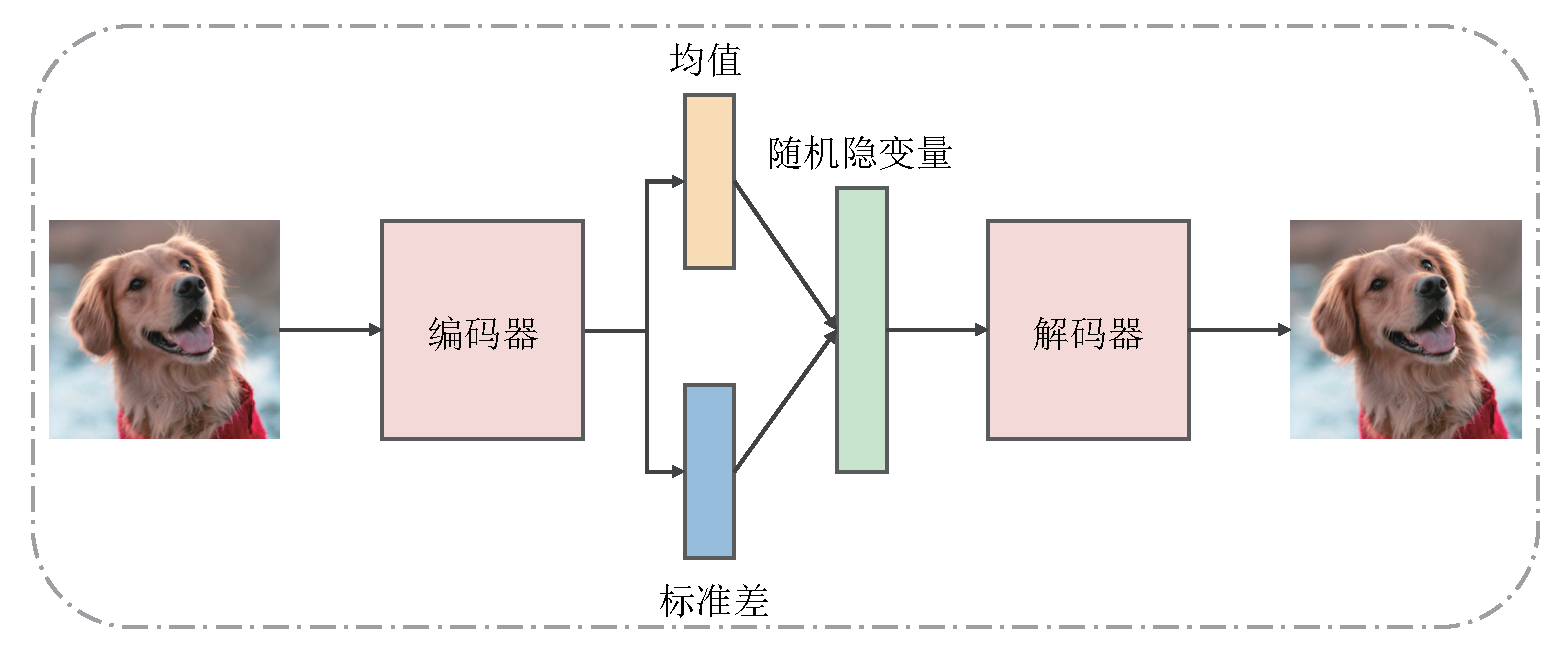
\includegraphics[width = \textwidth]{vae2}
\vspace{-1em}
\caption{变分自编码器结构 \label{vae}}
\end{figure}

\section{本文的主要研究内容}
本文主要研究了考虑缺失值对于时间分布和空间分布的影响的交通数据的算法设计问题。本文主要从以下三个方面,来对不完整的交通数据这一复杂的研究对象展开研究:

(1)时间依赖性:交通数据作为一种复杂的多维度时间数据。同一区域的交通状况在不同的时间点是呈现非线性的时间依赖关系,即是当前时刻的观测值和过去时刻的观测值是相互影响的,而不是独立的。同时,由于缺失值的存在的,使得同一区域中的时间数据可能是离散的,即是某一时刻的数值发生丢失,导致原本连续的时间数据变得零散。

(2)空间相关性:普通的交通数据的空间相关性,主要分为短距离的空间相关性,以及长距离的空间相关性。短距离的空间相关性主要是指某个地区交通流入量和邻近区域的交通流入量存在相关性;长距离的空间相关性主要是指由于交通设备的普及,某个区域的交通流入量会与较远区域的交通流入量存在相关性。同时,由于缺失值的存在,往往使得原本存在短距离空间相关性,或者长距离空间相关性发生丢失,导致以往的提取特征的方法效果往往会不好。

(3)缺失不确定性:由于内外因的干扰,交通数据的缺失现象是不可避免的,且数据缺失模式多样,缺失比例随机,这为数据补全带来了巨大的挑战。

针对以上挑战,本文在变分自编码器的基础上,首先设计了专门针对于带有缺失值的交通数据的时间特性的模块Biconvgrui,然后使用了针对于带有缺失值的交通数据的空间分布的卷积模块。且所设计方法实现了较低的填充绝对误差和相对误差。本文的研究工作围绕对于带有缺失值的交通数据的时间特性和空间特性的挖掘展开,具体内容如下:

(1)考虑缺失值对交通数据的时间分布特性影响的算法设计。考虑到城市交通网络可以按照经纬度划分为等距离的栅格图,那么在每个固定的时间区间内,该栅格图可视为包含多通道的图片,本文将一个城市内每日按照固定频率采集的栅格数据视为一段由多个连续帧组成的多通道视频,该处理方式能极大程度上保留原始交通数据的时空信息。同时,考虑到不同时间窗的交通数据会有不同的时间特性,因而选择小时周期,日周期以及周周期三种时间窗口划分交通数据集。在这个基础上,本文提出了一种可以处理多时间流的生成式填充神经网络模型(\textit{MTS-VAE})。该模型通过使用变分自编码器的强大的生成能力来填充交通数据的缺失值,通过学习随机隐变量的高斯分布来高度抽象交通数据的隐含信息。同时使用了多时间流窗口提取交通数据的不同周期的时间信息。为了充分提取包含缺失值的交通数据的时间分布,本文设计了一个特征提取模块,该模块中的Biconvgrui可以有效建模不完整交通数据的时间分布。同时,本文使用双向自注意力机制,增强卷积模块对于不完整数据中的缺失值和存在值的能力,并对提取的时空特征图在多个维度上进行校正。在开源交通数据集TaxiBJ、BikeNYC和TaxiNYC的实验结果表明,本文提出的填充模型\textit{MTS-VAE}在多种误差指标上都取得了优于主流填充算法的成绩。

(2)考虑缺失值对交通数据的空间分布特性影响的算法设计。虽然MTS-VAE模型使用了专门针对于带有缺失值的交通数据的时间特性的模块\textit{Biconvgrui},可以很好地建模不完整交通数据的时间分布。但是,考虑到缺失值的存在会使得交通数据的空间特性发生变化,使用普通的卷积模块很难有效地提取不完整数据的空间特征。同时,不同时间窗的交通数据间也是存在时间依赖性的,不能简单地将不同时间窗的交通数据视作相互独立的时间流数据。基于此,本文设计了一种多层Attention-Biconvgrui时空变分自编码器(\textit{MCST-VAE})。首先,该方法使用轻量级的双向注意力图的卷积模块替换原来的卷积模块,来达到能够动态更新掩膜的目的。其次,使用多层的Biconvgrui模型对三个时间窗(小时周期,日周期和周周期)的交通数据进行处理,得到一个包含大量存在信息的数据特征。最后,使用赛尔维斯特标准化流(Sylvester Normalizing Flows,SNFs)的变分自编码器替换基础的变分自编码器模型,使得模型可以通过学习随机隐变量的非高斯分布来高度抽象交通数据的隐含信息。最后,本文优化了模型的目标函数,使其不仅能填充输入数据的缺失值,且能保证高层语义信息的准确性。在上文提到的数据集上的实验结果显示,本文设计的模型\textit{MCST-VAE}的填充效果优于交通领域主流的算法,能够逐帧地对交通栅格数据进行精细化填充。
%,并且下游预测任务在使用此方法填充的数据集后能有效地提高预测的准确性
\section{本文的组织结构}

本论文一共分为四个章节。

第一章对本文的研究现状和研究背景进行详细的介绍。本章首先介绍了智能交通的基本理念,以及在智能城市中的重要地位,然后介绍了完整数据在智能交通应用中的重要性,进而强调对不完整的交通数据进行填充处理的必要性。随后介绍了国内外基于统计机器学习、神经网络和变分自编码器技术相关的缺失值填充算法的研究现状。最后重点描述了本文所面临的的一些挑战和主要的研究内容。

第二章阐述了研究本文所需要具备的相关理论基础和技术背景。本章节首先介绍了城市交通数据的一些相关的定义,同时对缺失数据的缺失机制进行了说明。然后对多种卷积操作进行介绍,并对Convgru模型进行说明。最后对目前较为流行的变分自编码器,以及其相关的延伸模型的原理进行介绍。通过本章相关知识的介绍,有助于读者理解第三、四章的算法设计内容。

第三章介绍了考虑时间缺失值分布特性的填充算法设计。本章先对现有的交通数据缺失值的填充算法进行介绍,分析了它们存在的不足之处。接着介绍了对于城市交通雷达数据的处理方式,随后提出了考虑了时间缺失值分布特性的多时间流变分自编码器的填充模型,并对模型的目标函数进行了详细的介绍。最后,本章介绍了所用的开源交通数据集、评价指标、实验设置,并对实验结果进行了分析总结。

第四章介绍了考虑空间缺失值分布特性的填充算法设计。本章节首先对上一章节的内容进行总结,并说明构建考虑空间缺失值分布特性的填充算法的必要性。接着提出了一种考虑空间缺失值分布特性的变分自编码器,并在传统的变分自编码器的基础上使用了标准化流编码器,以优化模型的生成效果。最后,本章分析了所提出了方法与对比方法的模型复杂度以及在公共数据集上的实验结果。

最后,结论部分对本文的研究内容和成果进行总结,对未来的可拓展研究的内容进行展望。

% Local Variables:
% TeX-master: "../thesis"
% TeX-engine: xetex
% End: